% vim:spelllang=ru,en
\documentclass[a4paper,12pt,notitlepage,headsepline,pdftex]{scrartcl}

\usepackage{cmap} % чтобы работал поиск по PDF
\usepackage[T2A]{fontenc}
\usepackage[utf8]{inputenc}
\usepackage[english,russian]{babel}
\usepackage{concrete}
\usepackage{cite}
\usepackage{url}

\usepackage{textcase}
\usepackage[pdftex]{graphicx}

\usepackage{lscape}

\pdfcompresslevel=9 % сжимать PDF
\usepackage{pdflscape} % для возможности альбомного размещения некоторых страниц
\usepackage[pdftex]{hyperref}
% настройка ссылок в оглавлении для pdf формата
\hypersetup{unicode=true,
            pdftitle={ПОЭВМ Лаба №6},
            pdfauthor={Погода Михаил},
            pdfcreator={pdflatex},
            pdfsubject={},
            pdfborder    = {0 0 0},
            bookmarksopen,
            bookmarksnumbered,
            bookmarksopenlevel = 2,
            pdfkeywords={},
            colorlinks=true, % установка цвета ссылок в оглавлении
            citecolor=black,
            filecolor=black,
            linkcolor=black,
            urlcolor=blue}

\usepackage{amsmath}
\usepackage{amssymb}
\usepackage{moreverb}
\usepackage{indentfirst}
\usepackage{misccorr}

\usepackage{xtab}
\usepackage{nccfoots}
\usepackage{listings}

\lstloadlanguages{C++}
\lstset{language=C++,basicstyle=\scriptsize,frame=tb,commentstyle=\itshape,stringstyle=\bfseries,extendedchars=false}
\begin{document}
\begin{titlepage}
  \begin{center}
    \large
    \MakeUppercase{Министерство образования и науки,}

    \MakeUppercase{молодёжи и спорта Украины}

    \mbox{\MakeUppercase{Национальный технический университет Украины}}

    \MakeUppercase{,,Киевский политехнический институт''}

    \addvspace{6pt}

    \normalsize
    Кафедра прикладной математики

    \vfill

    \textbf{Отчёт}

    Лабораторная работа \No 6

    по дисциплине ,,Программное обеспечение ЭВМ''

    \emph{,,Транспортная задача''}
  \end{center}

  \vfill

  \noindent
  \begin{minipage}{0.3\textwidth}
    Выполнил

    студент группы КМ-92

    Погода~М.\,В.
  \end{minipage}
  \hfill
  \begin{minipage}{0.4\textwidth}
    Проверила:

    Ковальчук"=Химюк~Л.\,А.
  \end{minipage}
  \vfill

  \begin{center}
    КИЕВ

    2012
  \end{center}
\end{titlepage}
\tableofcontents
\newpage
\section{Постановка задачи}
  В пунктах $S_1,\dots S_4$ производится некоторая продукция.
  Объём продукции задан в виде вектора $\vec{S}$.
  Продукция должна быть доставлена в пункты $D_1,\dots D_5$.
  Объём потребления также задан вектором.
  Также задана матрица стоимости перевозок из пункта $S_i$ в пункт $D_j$.

  \textit{Требуется} найти оптимальный план перевозок.
\section{Входные данные}
  \hfill\emph{Вариант~11}
  \begin{table}[h]
    \centering
    \begin{tabular}{|c|c|c|c|c||c|}
        \hline
        22 & 11 & 25 & 17 & 21 & 17\\
        \hline
        22 & 18 & 14 & 8 & 1 & 14\\
        \hline
        9 & 13 & 2 & 28 & 15 & 21\\
        \hline
        26 & 21 & 3 & 4 & 27 & 43\\
        \hline
        \hline
        19 & 22 & 23 & 17 & 14 & \\
        \hline
    \end{tabular}
    \caption{Условие}
    \label{tab:task}
  \end{table}
  \newpage
\section{Теоретические сведения}
  Для начала, необходимо найти опорное решение, которое затем оптимизируется,
  используя алгоритм метода потенциалов:
  \begin{enumerate}
    \item Взять любой опорный план перевозок, в котором отмечены $m + n - 1$
      базисных клеток (остальные клетки свободные).
    \item Определить для этого плана платежи ($a_i$ и $b_j$) исходя из
      условия, чтобы в любой базисной клетке псевдостоимости были равны
      стоимостям.
      Один из платежей можно назначить произвольно, например, положить равным
      нулю.
    \item Подсчитать псевдостоимости $c_{i,j} = a_i + b_j$ для всех свободных
      клеток.
      Если окажется, что все они не превышают стоимостей, то план
      \emph{оптимален}.
    \item Если хотя бы в одной свободной клетке псевдостоимость превышает
      стоимость, следует приступить к улучшению плана путём переброски
      перевозок по циклу, соответствующему любой свободной клетке с
      отрицательной ценой (для которой псевдостоимость больше стоимости).
    \item После этого заново подсчитываются платежи и псевдостоимости, и, если
      план ещё не оптимален, процедура улучшения продолжается до тех пор, пока
      не будет найден оптимальный план.
  \end{enumerate}

  \newpage
\section{Решение}
  \begin{table}[h]
    \centering
    \begin{tabular}{|c|c|c|c|c|}
      \hline
      0 & 17 & 0 & 0 & 0\\
      \hline
      0 & 0 & 0 & 0 & 14\\
      \hline
      19 & 2 & 0 & 0 & 0\\
      \hline
      0 & 3 & 21 & 17 & 0\\
      \hline
    \end{tabular}
    \caption{Решение}
    \label{tab:answer}
  \end{table}

  Цена полученного пути: 598.
\section{Описание программы}
  Программа написана на языке C++ с использованием библиотеки
  Qt\footnote{\url{http://qt-project.org}}.
  Программа ищет начальное базовое решение метотод наименьшего элемента, а
  затем оптимизирует его методом потенциалов.

  Пользователь имеет возможность просмотреть шаги оптимизации, т.\,е.
  промежуточные решения.
  \newpage
\section{Выводы}
  При выполнении данной лабораторной работы были реализованы метод
  минимального элемента и метод потенциалов, как методы решения транспортной
  задачи.

  Полученное решение является точным, т.\,к. метод потенциалов является
  модификацией симплекс"=метода, а симплекс"=метод является точным методом
  решения задач линейного программирования.
  \newpage
\section{Приложения}
  \subsection{Графическая форма приложения}
    \begin{figure}[h!]
      \begin{center}
        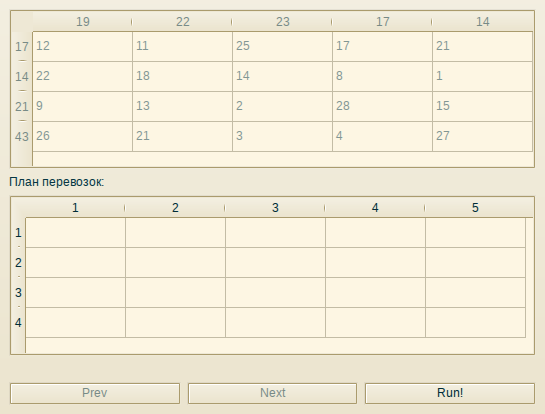
\includegraphics[width=\textwidth]{scr.png}
      \end{center}
      \caption{Графическая форма приложения}
      \label{fig:gui}
    \end{figure}
  \subsection{Исходные тексты}
    \subsubsection{CMakeLists.txt}
      \lstinputlisting{/home/projects/apps-for-computing/labd/CMakeLists.txt}
    \subsubsection{lab6\_widget.hxx}
      \lstinputlisting{/home/projects/apps-for-computing/labd/lab_widget.hxx}
    \subsubsection{lab6\_widget.cxx}
      \lstinputlisting{/home/projects/apps-for-computing/labd/lab_widget.cxx}
\end{document}
